\documentclass[tikz,border=10pt]{standalone}
\begin{document}
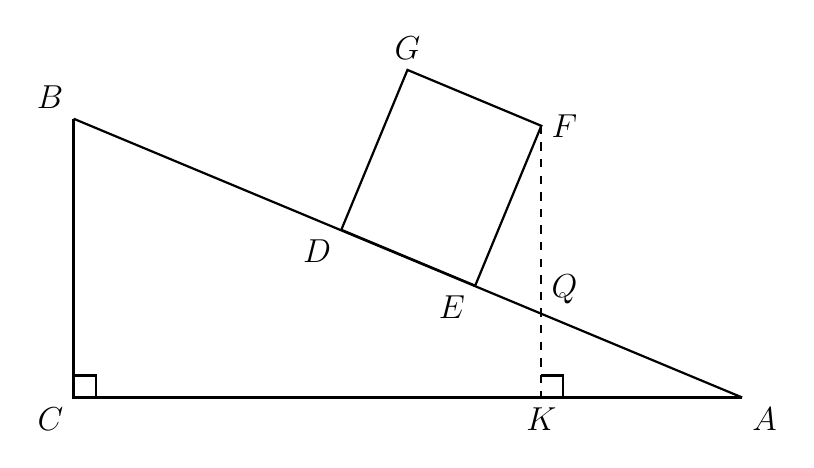
\begin{tikzpicture}[scale=1, line width=0.8pt, font=\large]
\coordinate (C) at (0,0);
\coordinate (B) at (0,3.54);
\coordinate (A) at (8.49,0);
\coordinate (K) at (5.94,0);
\coordinate (Q) at (5.94,1.06);
\coordinate (F) at (5.94,3.45);
\coordinate (G) at (4.24,4.16);
\coordinate (D) at (3.40,2.13);
\coordinate (E) at (5.10,1.42);

\draw (B) -- (A);
\draw (B) -- (C) -- (A);
\draw (D) -- (E) -- (F) -- (G) -- cycle;
\draw[dashed] (F) -- (K);

\draw (0,0.28) -- (0.28,0.28) -- (0.28,0);
\draw (5.94,0.28) -- (6.22,0.28) -- (6.22,0);

\node[above left] at (B) {$B$};
\node[below left] at (C) {$C$};
\node[below right] at (A) {$A$};
\node[below] at (K) {$K$};
\node[above right] at (Q) {$Q$};
\node[right] at (F) {$F$};
\node[above] at (G) {$G$};
\node[below left] at (D) {$D$};
\node[below left] at (E) {$E$};
\end{tikzpicture}
\end{document}
